
\section{Wu et al. (2020)}

% -------------------------------------------------------------------------

\begin{frame}
  \frametitle{Wu et al. (2020)}
  
  \begin{itemize}
  \item \textbf{Goal:} Study effect of long-term PM$_\text{2.5}$
    exposure on mortality rates \medskip 
  \item Estimand: $\E[Y(w)]$, where $Y$ is mortality rate per 100
    Medicare enrollees, and $w$ is PM$_\text{2.5}$ exposure in
    {\textmu}g/m$^\text{3}$
  \end{itemize}
  
\end{frame}

% -------------------------------------------------------------------------

\begin{frame}
  \frametitle{Local weak unconfoundedness}

  Treatment $W_j$ and covariates $\mathbf{C}_j$ \medskip 
  

    \begin{block}{\textit{Assumption}: Local weak unconfoundedness (Imbens, 2000)}
      $W_j \ind Y_j(w) \mid \mathbf{C}_j$ for all $w \in \mathcal{W}$ \smallskip

    \footnotesize \emph{Note: does not require joint independence of all
      potential outcomes $\{Y_j(w)\}_{w\in \mathcal{W}}$} \normalsize
  \end{block}

  Define the indicator variable $I_j(\tilde w) = 1$ if
  $W_j = \tilde w$ and $0$ otherwise.
  \begin{block}{\textit{Assumption}: Local weak unconfoundedness (Wu et al.)}
    $\{I_j(\tilde w)\}_{\tilde w \in [w-\delta, w+\delta]} \ind Y_j(w)
    \mid \mathbf{C}_j$ for all $z \in \mathcal{Z}$ \smallskip

    \footnotesize \emph{Note: this does not require joint independence of all
      potential outcomes $\{Y(z)\}_{z\in \mathcal{Z}}$} \normalsize
  \end{block}
  That is, the assignment is unconfounded \emph{within a neighborhood}
  of $w$ (not all $w \in \mathcal{W}$)

  \medskip Here $\delta$ is called the \textit{caliper}. 
  
\end{frame}

% -------------------------------------------------------------------------

\begin{frame}
  \frametitle{Matching with continuous treatments}
  
  \begin{itemize}
  \item Define a grid of values for $w$ \medskip 
  \item \textbf{Idea}: Match on both $w$ and the estimated GPS $e$,
    i.e. the objective function for matching is
    \begin{align*}
      m(e_j, w) = \arg \min_{k: w_k \in [w - \delta, w + \delta]}
      \| \lambda \cdot [e^\star(w_k, \mathbf{c}_k) - e^\star_j] +
      (1-\lambda) \cdot [w^\star_k - w^\star_j]\|
    \end{align*}
  \item The counterfactual outcome for unit $j$ at level treatment
    level $w$ is imputed as
    $\hat Y_j(w) = Y^{\text{obs}}_{m(e(w, \mathbf{c}_j), w)}$, i.e.,
    impute it from the unit close to $w$ (not $w_j$) and close in
    propensity score for unit $j$, $e_j$ \medskip
  \item Must select tuning parameters $\lambda$ and $\delta$ \medskip 
  \item Take average within each level of $w$, then use a kernel
    smoother to estimate the dose-response curve
  \end{itemize}


  
\end{frame}

% -------------------------------------------------------------------------

\begin{frame}
  \frametitle{Results on PM$_\text{2.5}$ mortality data} 
  
  \begin{figure}[ht]
    \centering
    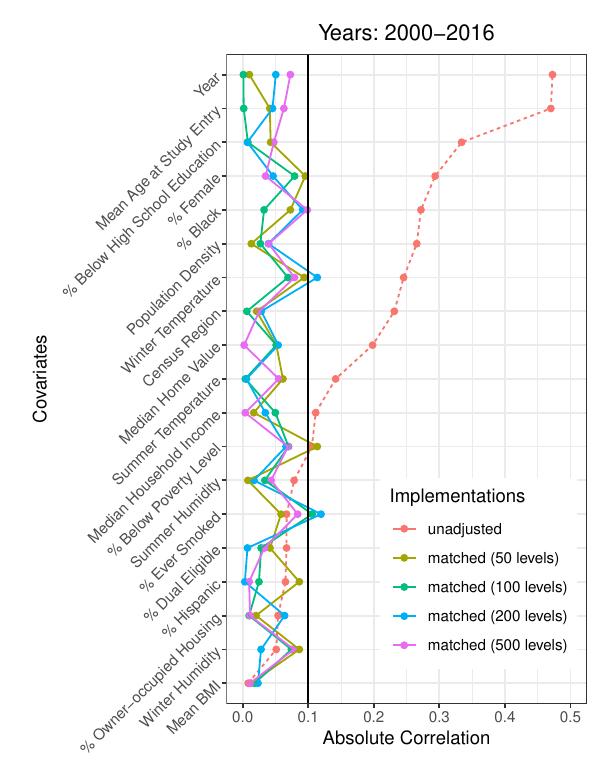
\includegraphics[height=0.8\textheight]{figures/wu-fig2.png}
  \end{figure}

  
\end{frame}

% -------------------------------------------------------------------------

\begin{frame}
  \frametitle{Results on PM$_\text{2.5}$ mortality data} 
  
  \begin{figure}[ht]
    \centering
    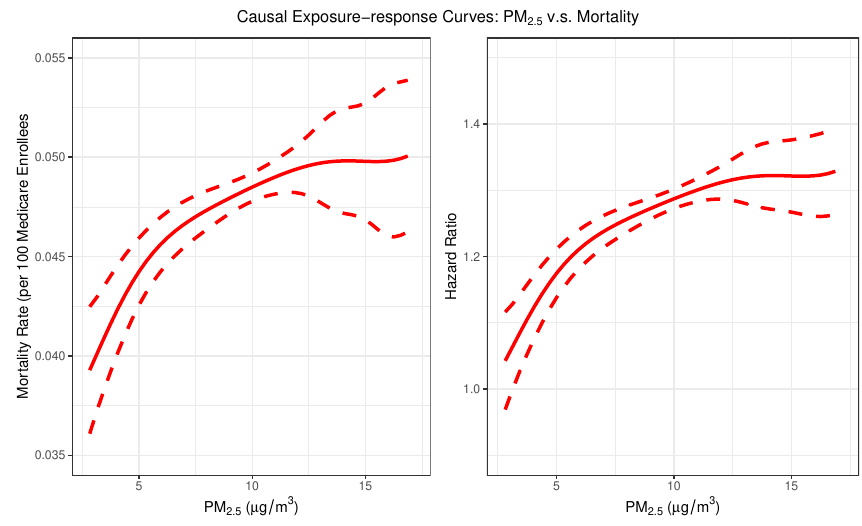
\includegraphics[width=\textwidth]{figures/wu-fig3.png}
  \end{figure}

  Confidence bands
  
\end{frame}


% -------------------------------------------------------------------------



\begin{frame}
  \frametitle{Open questions from Wu et al.}
  
  \begin{itemize}
  \item Is the bootstrap a valid way to represent uncertainty? \medskip 
  \item This method cannot estimate heterogeneous effects (e.g.,
    subgroups of the population)
  \end{itemize}
  
\end{frame}

%%% Local Variables:
%%% mode: latex
%%% TeX-master: "../main"
%%% End:
